%
% This is a borrowed LaTeX template file for lecture notes for CS267,
% Applications of Parallel Computing, UCBerkeley EECS Department.
% Now being used for CMU's 10725 Fall 2012 Optimization course
% taught by Geoff Gordon and Ryan Tibshirani.  When preparing 
% LaTeX notes for this class, please use this template.
%
% To familiarize yourself with this template, the body contains
% some examples of its use.  Look them over.  Then you can
% run LaTeX on this file.  After you have LaTeXed this file then
% you can look over the result either by printing it out with
% dvips or using xdvi. "pdflatex template.tex" should also work.
%

\documentclass[twoside]{article}
\setlength{\oddsidemargin}{0.25 in}
\setlength{\evensidemargin}{-0.25 in}
\setlength{\topmargin}{-0.6 in}
\setlength{\textwidth}{6.5 in}
\setlength{\textheight}{8.5 in}
\setlength{\headsep}{0.75 in}
\setlength{\parindent}{0 in}
\setlength{\parskip}{0.1 in}

%
% ADD PACKAGES here:
%

\usepackage{amsmath,amsfonts,graphicx}
\usepackage{minted}
\usepackage{mathtools}
%
% The following commands set up the lecnum (lecture number)
% counter and make various numbering schemes work relative
% to the lecture number.
%
\newcounter{lecnum}
\renewcommand{\thepage}{\thelecnum-\arabic{page}}
\renewcommand{\thesection}{\thelecnum.\arabic{section}}
\renewcommand{\theequation}{\thelecnum.\arabic{equation}}
\renewcommand{\thefigure}{\thelecnum.\arabic{figure}}
\renewcommand{\thetable}{\thelecnum.\arabic{table}}

%
% The following macro is used to generate the header.
%
\newcommand{\lecture}[4]{
   \pagestyle{myheadings}
   \thispagestyle{plain}
   \newpage
   \setcounter{lecnum}{#1}
   \setcounter{page}{1}
   \noindent
   \begin{center}
   \framebox{
      \vbox{\vspace{2mm}
    \hbox to 6.28in { {\bf UCSB CS 291D: Blockchains and Cryptocurrencies
	\hfill Fall 2020} }
       \vspace{4mm}
       \hbox to 6.28in { {\Large \hfill Lecture #1: #2  \hfill} }
       \vspace{2mm}
       \hbox to 6.28in { {\it Lecturer: #3 \hfill Scribes: #4} }
      \vspace{2mm}}
   }
   \end{center}
   \markboth{Lecture #1: #2}{Lecture #1: #2}

%   {\bf Note}: {\it LaTeX template courtesy of UC Berkeley EECS dept.}

%   {\bf Disclaimer}: {\it These notes have not been subjected to the
%   usual scrutiny reserved for formal publications.  They may be distributed
%   outside this class only with the permission of the Instructor.}
%   \vspace*{4mm}
}
%
% Convention for citations is authors' initials followed by the year.
% For example, to cite a paper by Leighton and Maggs you would type
% \cite{LM89}, and to cite a paper by Strassen you would type \cite{S69}.
% (To avoid bibliography problems, for now we redefine the \cite command.)
% Also commands that create a suitable format for the reference list.
\renewcommand{\cite}[1]{[#1]}
\def\beginrefs{\begin{list}%
        {[\arabic{equation}]}{\usecounter{equation}
         \setlength{\leftmargin}{2.0truecm}\setlength{\labelsep}{0.4truecm}%
         \setlength{\labelwidth}{1.6truecm}}}
\def\endrefs{\end{list}}
\def\bibentry#1{\item[\hbox{[#1]}]}

%Use this command for a figure; it puts a figure in wherever you want it.
%usage: \fig{NUMBER}{SPACE-IN-INCHES}{CAPTION}
\newcommand{\fig}[3]{
			\vspace{#2}
			\begin{center}
			Figure \thelecnum.#1:~#3
			\end{center}
	}
% Use these for theorems, lemmas, proofs, etc.
\newtheorem{theorem}{Theorem}[lecnum]
\newtheorem{lemma}[theorem]{Lemma}
\newtheorem{proposition}[theorem]{Proposition}
\newtheorem{claim}[theorem]{Claim}
\newtheorem{corollary}[theorem]{Corollary}
\newtheorem{definition}[theorem]{Definition}
\newenvironment{proof}{{\bf Proof:}}{\hfill\rule{2mm}{2mm}}

% **** IF YOU WANT TO DEFINE ADDITIONAL MACROS FOR YOURSELF, PUT THEM HERE:

\newcommand\E{\mathbb{E}}

\begin{document}
%FILL IN THE RIGHT INFO.
%\lecture{**LECTURE-TITLE**}{**DATE**}{**LECTURER**}{**SCRIBE**}
\lecture{12}{zkSnark Internals II}{Shumo Chu}{Rakshith Gopalakrishna}
%\footnotetext{These notes are partially based on those of Nigel Mansell.}

% **** YOUR NOTES GO HERE:

% Some general latex examples and examples making use of the
% macros follow.  
%**** IN GENERAL, BE BRIEF. LONG SCRIBE NOTES, NO MATTER HOW WELL WRITTEN,
%**** ARE NEVER READ BY ANYBODY.



In the last class we studied how to perform the blind evaluation of polynomials and the Knowledge Coefficient Test and Assumption. 
To recap, suppose that Alice has a polynomial $P$ of degree $d$, and Bob has a point $s \in \mathbb{F}_p$ and let $E$ be a homomorphic hiding.
We want Alice to \emph{blindly} evaluate the polynomial $P$ at point $s$ and return $E(P(s))$ to Bob. KCA states that if Alice responds with the 
pair 
$(a', b')$ to Bob's challenge $(a, b)$ with non-negligible probablity over Bob's choices of $a, \alpha$, then she knows a $\gamma$ such
that $a' = \gamma a$ and $b' = \gamma b$.

{\bf Properties of blind evaluation}

We require these two properties of blind evaluation.
\begin{enumerate}
\item Blindness -- Alice should not learn $s$ and Bob should not learn $P$.
\item Verifiability -- The probability that Alice sends a value different from $E(P(s))$ for a $P$ of degree $d$ 
that is still accepted by Bob is negligible.
\end{enumerate}

Recall that the polynomial $P$ is defined as $$P(x) = a_0x^{0} + a_1x + a_2x^2 + \dots + a_dx^d$$
In short, $P$ is defined by the coefficients
$\lbrack a_0, a_1, \dots , a_d \rbrack$

One natural way to think of arriving at verifiable blind evaluation of polynomials is to extend the KCA protocol to use $d$ $\alpha$-pairs.
Essentially repeating the KCA protocol $d$ times so that we can handle the encoding of $d$ coefficients in the polynomial $P$.

\section{An Extended KCA}
As discussed above, one could run the KCA protocol $d$ times to achieve verifiable blind evaluation. However, the communication cost 
is very high. Ideally we want Alice to send back to Bob a single $\alpha$-pair that can verify all the $d$ $\alpha$-pairs that Bob 
sends to Alice. If Bob can verify this single $\alpha$-pair instead of repeating this for $d$ rounds, we arrive at a communication efficient
protocol. Notice that Alice can take any linear combination of the given $d$ pairs and define her $\alpha$-pair as 
$(a', b') = (\Sigma_{i=1}^{d} c_ia_i, \Sigma_{i=1}^{d} c_ib_i)$ for any $c_1, \ldots, c_d \in \mathbb{F}_p$. 

In other words, if Bob sends $d$ $\alpha$-pairs to Alice, Alice only needs to send back a linear combination of the pairs back to Bob 
to prove that she knows some linear relation between the $d$ pairs. This is the d-KCA protocol. 

More formally, suppose Bob samples $d$ $\alpha$-pairs $(a_1, b_1), \ldots, (a_d, b_d)$ at random and sends these $\alpha$-pairs to Alice.
Suppose that Alice sends back a single $\alpha$-pair $(a', b')$. Then, except with negligible probability, Alice knows 
$c_1, \ldots, c_d \in \mathbb{F}_p$ such that $\Sigma_{i=1}^{d} c_ia_i = a'$.


\section{Verifiable Blind Evaluation protocol}
Assume that the homomorphic hiding $HH$ is the mapping $E(x) = x \cdot g$ for a generator $g$ of a group $G$ of size $p$.
\begin{enumerate}
\item Bob chooses $\alpha \xleftarrow{\$} D$ and constructs the $\alpha$-pairs 
$(E(1), \alpha E(1)), (E(s), \alpha E(s)), \ldots, (E(s^d), \alpha E(s^d))$ and sends these to Alice.
\item Alice computes $a' = E(P(s)) = P(s) \cdot g$ and $b = \alpha E(P(s)) = \alpha P(s) \cdot g$ and sends this $\alpha$ pair
to Bob.
\item Bob checks that $b' = \alpha \cdot a'$ and accepts $(a;, b')$ iff this equality holds.
\end{enumerate}

This protocol is provides blind evaluation of a polynomial as long as d-KCA is true.

\section{Expressing computations as polynomials}
Quadratic Arithmetic Programs (QAP) are the extremely useful translation of computations into polynomials. They form the basis
of modern zk-SNARK constructions.

Suppose that Alice wants to prove to Bob that she knows the satisfying assignment for the equation $x^3 + x + 5 = 35$. 
The computation here is the function $f(x) = x^3 + x + 5$. One could represent this function in the form of the following 
python program.
\begin{minted}{python}
def f(x):
    y = x**3
    return x + y + 5
\end{minted}

In order to represent this computation as a polynomial, we need to go through the intermediate steps of representing them as
arithmetic circuits, R1CS and finally QAP.

\subsection{Computation to arithmetic circuit}
First step is to flatten the program into so that all operations are of the form $var_1 = var_2 <op> var_3$ where $op = +, -, *, /$.
In the process of doing this, we can also introduce as many intermediate values as required. This step is very similar to 
Single Static Assignment used in compilers.

Our flattened program looks like this. Note that the variables once defined are immutable.

\begin{minted}{python}
sym_1 = x * x
y = sym_1 * x
sym_2 = y + x
~out = sym_2 + 5
\end{minted}

From the flattened program, we can now construct an arithmetic circuit by replacing each variables on the left, right and the operator with
output of a gate, input to a gate and an arithmetic gate respectively.

The arithmetic circuit for the given program is given in figure \ref{f:circuit}.

\begin{figure}
\centering
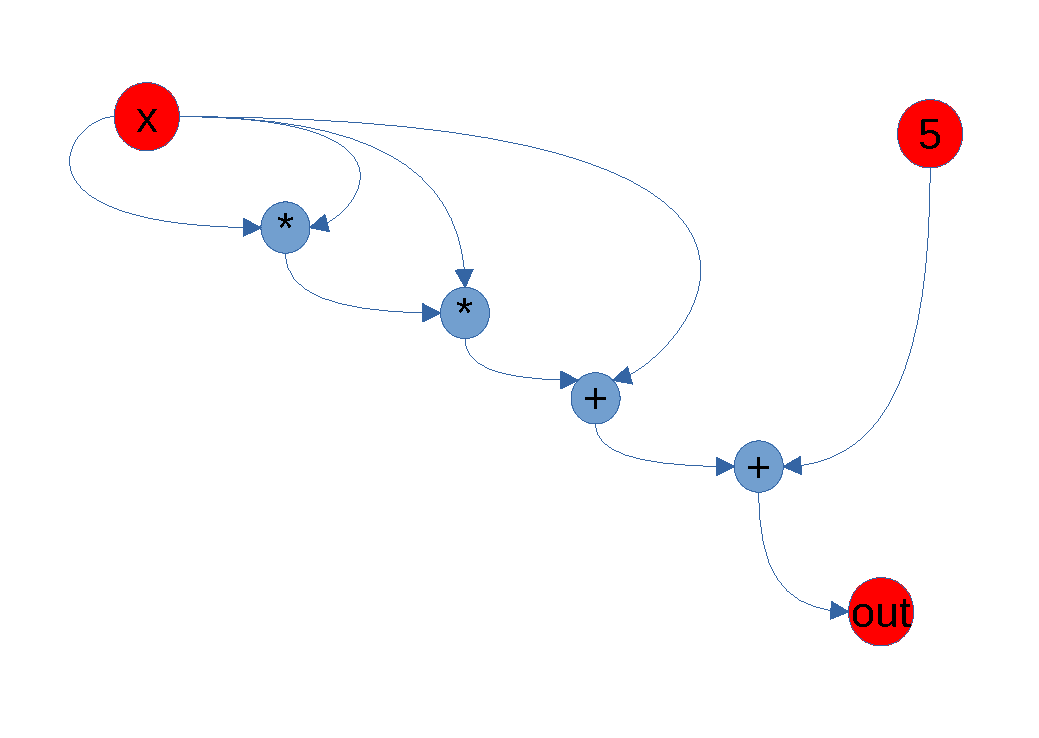
\includegraphics[width=0.75\textwidth]{lecture12-circuit.pdf}
\caption{Arithmetic circuit for the computation $x^3 + x + 5$}
\label{f:circuit}
\end{figure}




\subsection{Circuit to R1CS}
We define the vector $C$ to denote the assignment to the variables used in the program. 
Let $C = \lbrack \sim one, x, \sim out, sym\text{\_}1, y, sym\text{\_}2 \rbrack$.
Let $C_0$ denote the concrete assignment to the variables. For instance, $C_0 = \lbrack 1, 5, 7, 8, 6, 10\rbrack$.

R1CS is a sequence of groups of three vectors $(l, r, o)$. Suppose $c$ is the concrete assignment to the variables, the computation in each 
gate should obey the following format
$$<c.l> \times <c.r> = <c.o>$$ where $<.>$ denotes the inner product of two vectors.

Let us now visualize how each line in the flattened program can be represented in the R1CS form.

\begin{enumerate}
\item
{\bf $sym\text{\_}1 = x \times x$}


$$ l = \lbrack 0, 1, 0, 0, 0, 0 \rbrack $$ 
$$ r = \lbrack 0, 1, 0, 0, 0, 0 \rbrack $$
$$ o = \lbrack 0, 0, 0, 1, 0, 0 \rbrack $$


\item 
{\bf $sym\text{\_}1 * x = y$}

$$ l = \lbrack 0, 0, 0, 1, 0, 0 \rbrack $$ 
$$ r = \lbrack 0, 1, 0, 0, 0, 0 \rbrack $$
$$ o = \lbrack 0, 0, 0, 0, 1, 0 \rbrack $$

\item 
{\bf $y + x = sym\text{\_}2$}

$$ l = \lbrack 0, 1, 0, 0, 1, 0 \rbrack $$ 
$$ r = \lbrack 1, 0, 0, 0, 0, 0 \rbrack $$
$$ o = \lbrack 0, 0, 0, 0, 0, 1 \rbrack $$

\item
{\bf $sym\text{\_}2 + 5 = \sim out$}

$$ l = \lbrack 5, 0, 0, 0, 0, 1 \rbrack $$ 
$$ r = \lbrack 1, 0, 0, 0, 0, 0 \rbrack $$
$$ o = \lbrack 0, 0, 1, 0, 0, 1 \rbrack $$

\end{enumerate}

Now that we have an R1CS with four constraints, the witness is simply the assignment to all variables including the input, output 
and intermediate variables.


\subsection{R1CS to QAP}
The next step is to convert the R1CS into QAP form. In order to do this, we go from four groups (for the four gates) of three vectors
of length 6 (for 6 variables) to six groups of three degree-3 polynomials where evaluating the polynomimals at each $x$ represents one of the
constraints.

Let $L(x)^{T} = \lbrack L_1(x), L_2(x), \ldots, L_6(x) \rbrack$, $R(x)^{T} = \lbrack R_1(x), R_2(x), \ldots, R_6(x) \rbrack$ and 
$O(x)^{T} = \lbrack O_1(x), O_2(x), \ldots, O_6(x) \rbrack$. 

Rewriting the R1CS for the arithmetic circuit 
$C\cdot L(x) \times C\cdot R(x) - C\cdot O(x) = 0$ as equation \ref{e:QAP}

\begin{align}
C \cdot \begin{bmatrix}
L_1(x) \\
L_2(x) \\
\vdots \\
L_6(x)
\end{bmatrix} ~\times~  C \cdot \begin{bmatrix}
R_1(x) \\
R_2(x) \\
\vdots \\
R_6(x)
\end{bmatrix} ~-~ C\cdot \begin{bmatrix}
O_1(x) \\
O_2(x) \\
\vdots \\
O_6(x)
\end{bmatrix} = 0
\label{e:QAP}
\end{align}

helps us visualize the QAP. Each row can be considered a group of polynomials and this is how we arrive at 
six groups of three degree-3 polynomials.

We can find out the the coefficients of the polynomials $L_1, \ldots, L_6, R_1, \ldots, R_6, O_1, \ldots, R_6$ using Lagrange interpolation.
Essentially, given a set of points, Lagrange interpolation allows us to construct a polynomials that passes through all of them.
Suppose we want a polynomial that passes through $(1, 3), (2, 2)$ and $(3, 4)$. We can start by constructing a polynomial that passes through
$(1, 3), (2, 0), (3, 0)$, a second polynomial that passes through $(1, 0), (2, 2), (3, 0)$ and a third polynomial that passes
through $(1, 0), (2, 0), (3, 4)$. Now, adding these polynomials gives us the required polynomial that passes through all the points.


\section{Quadratic Arithmetic Program}

A quadratic arithmetic program $Q$ of degree $d$ and size $m$ consists of polynomials $L_1, \ldots, L_m, R_1, \ldots, R_m, O_1, \ldots, O_m$,
a target polynomial $T$ of degree $d$.
Define $L \coloneqq \Sigma_{i=1}^{m} c_i\cdot L_i$, $R \coloneqq \Sigma_{i=1}^{m} c_i\cdot R_i$ and $O \coloneqq \Sigma_{i=1}^{m} c_i\cdot O_i$ and then 
define $P \coloneqq L \cdot R - O$. An assignment $(c_1, \ldots, c_m)$ satisfies $Q$ iff T divides P.



% **** THIS ENDS THE EXAMPLES. DON'T DELETE THE FOLLOWING LINE:

\end{document}

